\section{Versuchsdurchführung}

The goal is to determine the maximum resolution of a microscope.

The experiment will be split into three experiments:

\begin{enumerate}
	\item{Experiment: Fixing the tube length to the best distance to get the calculated magnification.}
	\item{Experiment: Determining the lattice constant d by measuring the width of the gap and the thickness of a wire from a grid.}
	\item{Experiment: Determining the maximum resolution of the microscope by using an adjustable pinhole.}
\end{enumerate}

For the first experiment a microscope was needed to be prepared as shown in illustration 1.  The goal was to find the right distance for the tube length to match the calculated magnification. A lamp with a scale placed at the end, which had a wavelength of 550nm. With some distance the objective lens (f\_ok=50mm) was placed. Behind the objective lens the ocular lens (f\_ob=50mm) was placed. The tube had a length of 100mm. A semi-transparent mirror was placed in front of the ocular in an 45° angle, to show a second scale (same size as the scale on the lamp), which was s\_0=250mm away. It was also necessary to keep the distance from the ocular to the eye at s\_0, to see a clear image.
\\
By trial and error, the optimal distance x=25cm from the lamp to the objective lens was found. At this point the theoretical magnification (equation X) and the measurement (equation X) came booth to two. The magnification was calculated by equation X. To check the correctness, the experiment was repeated two more times (x=25cm ) with the tube length changed to 150mm and 200mm.

\begin{figure}[h!]
    \centering
  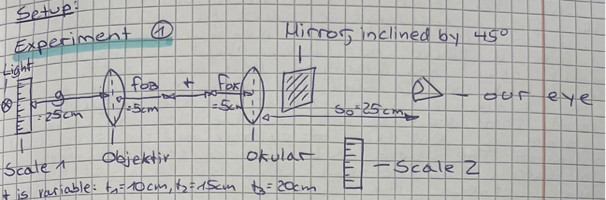
\includegraphics[]{Illu1_Experiment_setup_1.jpg}
  \caption{Setup of experiment 1}
\end{figure}

In experiment 2 a grid was now placed in front of the lamp and the tube length changed to 300mm to get a sufficient magnification. An ocular micrometre (graduation: 1,33 $\pm$ 0,06 $\cdot10^{-9}$ mm) in the focal point of the ocular lens was needed to measure the gaps and the thickness of the wires from the grid.

As last step of the experiment, the ocular micrometre was switched with an adjustable pinhole. By changing the pinhole size, it was possible to determine the resolution limit.

\begin{figure}[h!]
    \centering
  \includegraphics[]{Illu2_Experiment_setup_3.jpg}
  \caption{Setup of experiment 3}
\end{figure}

\newpage
